% %% ========================================
\section{Proposed Solution}\label{sec:solution}

The unified framework called PushAround is developed to enable collaborative multi-robot pushing
with physical feasibility, as described in this section.
The framework begins by constructing a
W-Clearance Connectivity Graph, introduced in Sec.~\ref{subsec:wccg}, which
captures the connectivity of the workspace under the clearance requirement
and identifies frontier gaps that block passage. Building on this
representation, Sec.~\ref{subsec:gap} presents a gap-ranking strategy that
assigns costs to candidate gaps and determines which obstacle-clearing actions
are most promising. These ranked actions are then evaluated within a
simulation-in-the-loop search, described in Sec.~\ref{subsec:simloop}, where a
configuration-space tree is expanded and candidate pushes are validated by
parallel physical simulation. The complete execution flow together with
generalization aspects is summarized in Sec.~\ref{subsec:overall}.



% %% ========================================
%------------------------------
\begin{figure*}[t!]
  \centering
  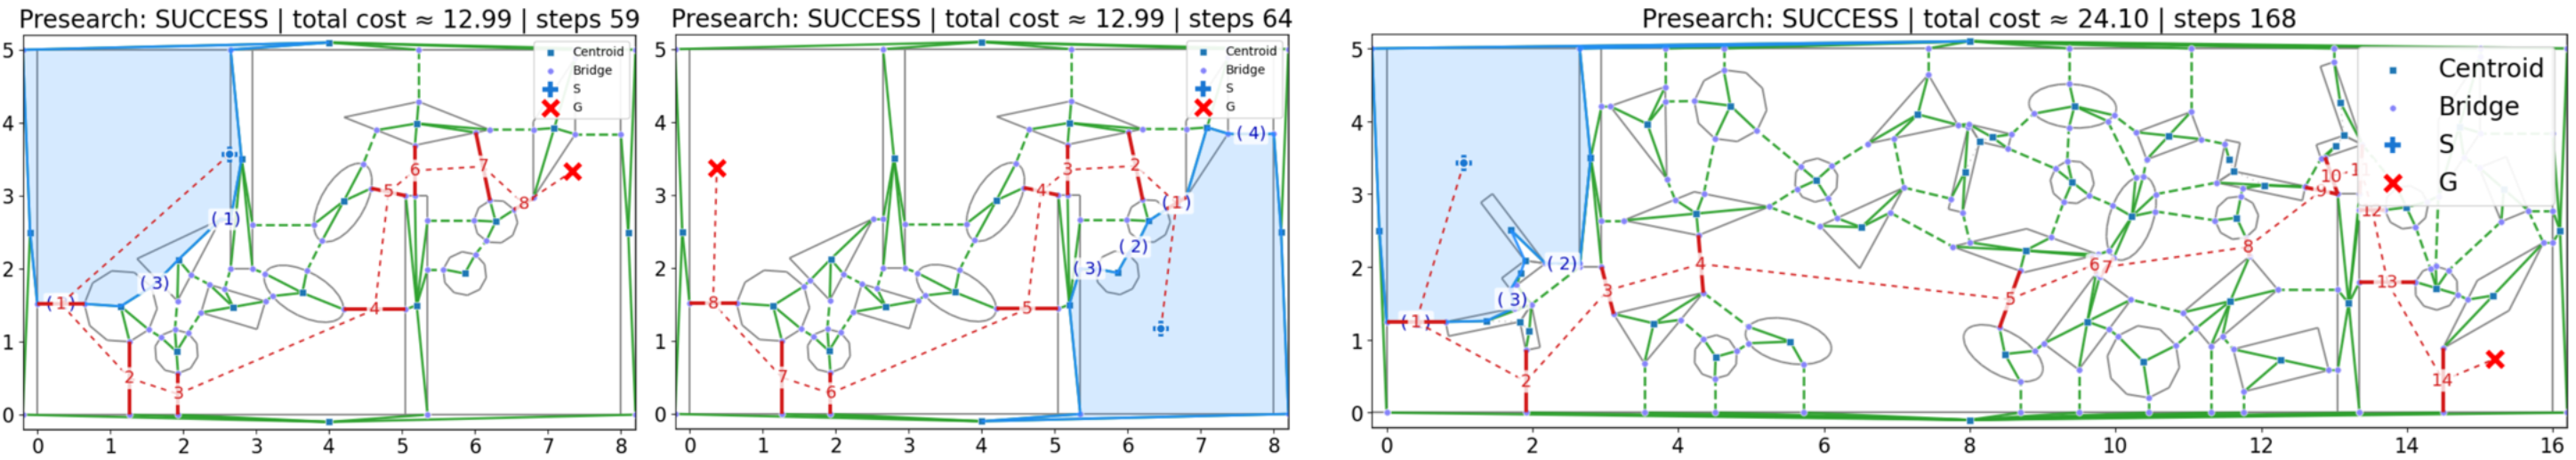
\includegraphics[width=0.95\linewidth]{figures/presearch.png}% or {presearch.pdf}
  \vspace{-0.15in}
\caption{
Illustration for {the ranking of potential gaps.}
Each panel shows the WCCG with the current face (light blue).
The algorithm (i) extracts the frontier loop from BugPlanner,
(ii) enumerates candidate bridge--bridge gaps on the loop,
(iii) assigns local first-hop ranks (blue numbers),
and (iv) simulates a short presearch to predict the full gap-crossing sequence (red numbers).
\textbf{Top}: start and goal swapped in the same map give symmetric
sequences with cost $12.99$;
\textbf{Right}: a larger map with about 30 obstacles produces a 14-gap sequence
with cost $24.10$.
}
  \label{fig:presearch}
   \vspace{-4mm}
\end{figure*}
%------------------------------
%==============================================
\subsection{W--Clearance Connectivity Graph}\label{subsec:wccg}

The feasibility of routing the vehicle reduces to whether a width-$W$ corridor 
connects $\mathbf{s}_\texttt{V}^{\texttt{S}}$ and $\mathbf{s}_\texttt{V}^{\texttt{G}}$. 
We introduce a W--Clearance Connectivity Graph (WCCG; Fig.~\ref{fig:wccg}) 
that encodes obstacle adjacencies under clearance $W$ and enables fast connectivity queries. 
Constructed directly from geometry (rather than grids/roadmaps), 
it avoids discretization error and remains consistent—crucial because connectivity is checked repeatedly 
during planning.

\subsubsection{Graph Construction}
The WCCG is built by decomposing each movable obstacle
$\Omega_m\in\boldsymbol{\Omega}$ into convex components. From each component
$C$, a centroid node $v_c$ is created. When two components $C_u$ and $C_v$
have closest points $p_u\in C_u$ and $p_v\in C_v$ with distance less than $W$, 
bridge nodes are added at $p_u$ and $p_v$. These bridge nodes are
connected by a bridge--bridge edge, annotated with the corresponding gap width
$w_{uv}\triangleq\|p_u-p_v\|$, and further linked back to their centroids with
centroid--bridge edges. Narrow passages with $w_{uv}<W$ are explicitly marked
as potential bottlenecks. The resulting graph is defined below:
\begin{equation}\label{eq:wccg}
\mathcal{G}_W\triangleq(\mathcal{V},\; \mathcal{E}_c\cup\mathcal{E}_b),
\end{equation}
where $\mathcal{V}$ contains all centroid and bridge nodes;
$\mathcal{E}_c$ is the set of centroid--bridge edges; and $\mathcal{E}_b$ the
set of bridge--bridge edges annotated by widths $w_{uv}$.

\subsubsection{Connectivity Criterion}\label{subsubsec:bugplanner}
Once $\mathcal{G}_W$ has been constructed, connectivity queries can be
performed without explicitly computing a geometric path. A frontier-tracing
procedure, similar to the BugPlanner~\cite{McGuireCroonTuyls2019}, starts from the vehicle start
$\mathbf{s}_\texttt{V}^{\texttt{S}}$, casts a ray toward the goal
$\mathbf{s}_\texttt{V}^{\texttt{G}}$, and explores the encountered loop of
frontier edges. If a valid exit is discovered, the process continues until the
goal is reached; otherwise a blocking cycle is returned. Successful execution
produces a skeleton $\Sigma$, which is an ordered sequence of centroid and
bridge nodes that certifies $\mathbf{s}_\texttt{V}^{\texttt{S}}$ and
$\mathbf{s}_\texttt{V}^{\texttt{G}}$ lie in the same connected face.
Let the $W$--clear free space be
$\mathcal{F}_W\triangleq\mathbb{R}^2\setminus(\mathcal{O}\oplus\mathbb{B}_{W/2})$,
where $\oplus$ denotes Minkowski addition and $\mathbb{B}_{W/2}$ is a closed
disk of radius $W/2$. A complete criterion for existence of a $W$--clear path
$\mathcal{P}^W_\texttt{V}$ is defined as:
\begin{equation}\label{eq:wccg_criterion}
\begin{aligned}
&\exists\,\mathcal{P}^W_\texttt{V}\subset\mathcal{F}_W:\
  \mathbf{s}_\texttt{V}^{\texttt{S}}\leadsto\mathbf{s}_\texttt{V}^{\texttt{G}} \Longleftrightarrow\
  \Big{\{}\mathbf{s}_\texttt{V}^{\texttt{S}},\mathbf{s}_\texttt{V}^{\texttt{G}}
  \ \text{belong to the} \\
  & \text{same face of }\mathcal{G}_W; \;\mathbb{B}_{W/2}(\mathbf{s}_\texttt{V}^{\texttt{S}}),
  \,\mathbb{B}_{W/2}(\mathbf{s}_\texttt{V}^{\texttt{G}})\subset\mathcal{F}_W\Big{\}},
\end{aligned}
\end{equation}
where $\mathbb{B}_{W/2}(\cdot)$ denotes a disk of radius $W/2$ centered at the
argument. This aligns with~\eqref{eq:wclear} for the external vehicle.

\subsubsection{Skeleton to Path}
The skeleton~$\Sigma$, the output of the previous step,
is an ordered sequence of centroid and bridge nodes connected by frontier
edges in $\mathcal{G}_W$. This skeleton serves as a compact certificate that
$\mathbf{s}_\texttt{V}^{\texttt{S}}$ and $\mathbf{s}_\texttt{V}^{\texttt{G}}$
lie in the same connected face. Given as input the skeleton $\Sigma$, together
with $\mathcal{G}_W$, the clearance $W$, and the endpoint disks
$\mathbb{B}_{W/2}(\mathbf{s}_\texttt{V}^{\texttt{S}})$ and
$\mathbb{B}_{W/2}(\mathbf{s}_\texttt{V}^{\texttt{G}})$, the output is an explicit
$W$--clear path $\mathcal{P}^W_\texttt{V}$. This path is constructed by sliding
each skeleton segment along the boundary of the inflated obstacles, offsetting
slightly inward into $\mathcal{F}_W$, and attaching short connectors inside the
endpoint disks. The resulting $\mathcal{P}^W_\texttt{V}$ remains in
$\mathcal{F}_W$, preserves the homotopy of $\Sigma$, and guarantees clearance of
at least $W$.


\begin{remark}\label{remark:wccg}
  The proposed WCCG differs from sampling- and grid-based planners in two key aspects:
  (I) It avoids discretization of $\mathcal{W}$ and is therefore free from
  resolution-induced errors;
  (II) It relies purely on geometry, which makes
queries highly efficient. These two features are crucial, since connectivity
checks and clearance tests are invoked many times within the hybrid
planner described in the sequel. \hfill$\blacksquare$
\end{remark}





%% \begin{algorithm}[t!]
%% \small
%% \caption{BugPlanner for $W$-width connectivity (skeleton witness)}
%% \label{alg:bugplanner}
%% \DontPrintSemicolon
%% \SetKwInOut{Input}{In}\SetKwInOut{Output}{Out}
%% \Input{$\mathbf{s}^{\texttt{S}}$, $\mathbf{s}^{\texttt{G}}$, WCCG}
%% \Output{if connected: skeleton $\Sigma$; else: frontier loop $\mathcal{L}$}
%% $P\leftarrow\mathbf{s}^{\texttt{S}}$, $\Sigma\leftarrow[\ ]$\;
%% \While{true}{
%%   \If{segment $P\mathbf{s}^{\texttt{G}}$ hits no edge}{\Return $\Sigma \cup \{\texttt{straight}(P,\mathbf{s}^{\texttt{G}})\}$}
%%   Build loop $\mathcal{L}$ by angle-follow from the hit edge; append traversed edges to $\Sigma$\;
%%   \If{$\mathrm{parity}(\mathcal{L},\,\mathbf{s}^{\texttt{S}}\mathbf{s}^{\texttt{G}})$ is odd}{\Return $(\emptyset,\mathcal{L})$}
%%   Choose exit $e$ on $\mathcal{L}$ (outward normal $\to\,\mathbf{s}^{\texttt{G}}$); append arc to $\Sigma$; $P\leftarrow e$ (tiny bias)\;
%% }
%% \end{algorithm}

% %% ========================================
%==============================================
\subsection{Ranking of Potential Blocking Gaps}\label{subsec:gap}

When the condition in~\eqref{eq:wccg_criterion} fails, the vehicle cannot
reach~$\mathbf{s}_\texttt{V}^{\texttt{G}}$ from
$\mathbf{s}_\texttt{V}^{\texttt{S}}$ through a $W$--clear path
$\mathcal{P}^W_\texttt{V}$. In this case, the planner must prioritize
\emph{blocking gaps} on the reachable frontier of $\mathcal{G}_W$. The goal of
this module is to provide an ordered list of such gaps, ranked by their
predicted cost to eventually yield a feasible path, which serves
as a critical guidance for the hybrid search in the sequel.

\subsubsection{Frontier Extraction and Candidate Gaps}
A BugPlanner query on $\mathcal{G}_W$, given
$(\mathbf{s}_\texttt{V}^{\texttt{S}},\mathbf{s}_\texttt{V}^{\texttt{G}},W)$,
either confirms connectivity or returns a counter--clockwise frontier loop
$\mathcal{L}$ that separates the two endpoints. The bridge--bridge edges
visible on $\mathcal{L}$ form the first--hop candidate set
$\Gamma_\mathcal{L}\triangleq\{g_1,\cdots,g_K\}$,
where each $g_k$ is a reachable candidate gap. These candidates are the inputs
to the ranking module, while the output will be an ordered list of the same
set sorted by predicted cost.

\subsubsection{Evaluation for Immediate Cost}
Each candidate $g\in\Gamma_\mathcal{L}$ is evaluated by combining the
cost for the robots to reach the gap and the effort required to widen it.
Let $\mathbf{s}_{\mathcal{R}}$ be the current robot positions,
and $\mathbf{o}_g$ as the outside insertion point of gap $g$. The
resulting one--hop cost is given by:
\begin{equation}\label{eq:step_cost}
\mathsf{C}\big(g \mid \mathcal{L}, \mathbf{s}_{\mathcal{R}}\big)
=\lambda_\texttt{t}\,\mathsf{C}_\texttt{t}\!\left(\mathbf{s}_{\mathcal{R}},\mathbf{o}_g\right)
+\lambda_\texttt{p}\,\mathsf{C}_\texttt{p}(g),
\end{equation}
where $\lambda_\texttt{t},\lambda_\texttt{p}>0$ are weighting factors
for the transition and pushing costs, respectively;
function $\mathsf{C}_\texttt{t}(\cdot)$ denotes the collision-free
distance between two points;
and the function~$\mathsf{C}_\texttt{p}(\cdot)$ measures the widening effort,
which increases when the gap is narrower than $W$,
or when the adjacent obstacles are heavier as scaled by the  mass of adjacent movable
obstacles.

%------------------------------
\begin{figure}[t!]
  \centering
  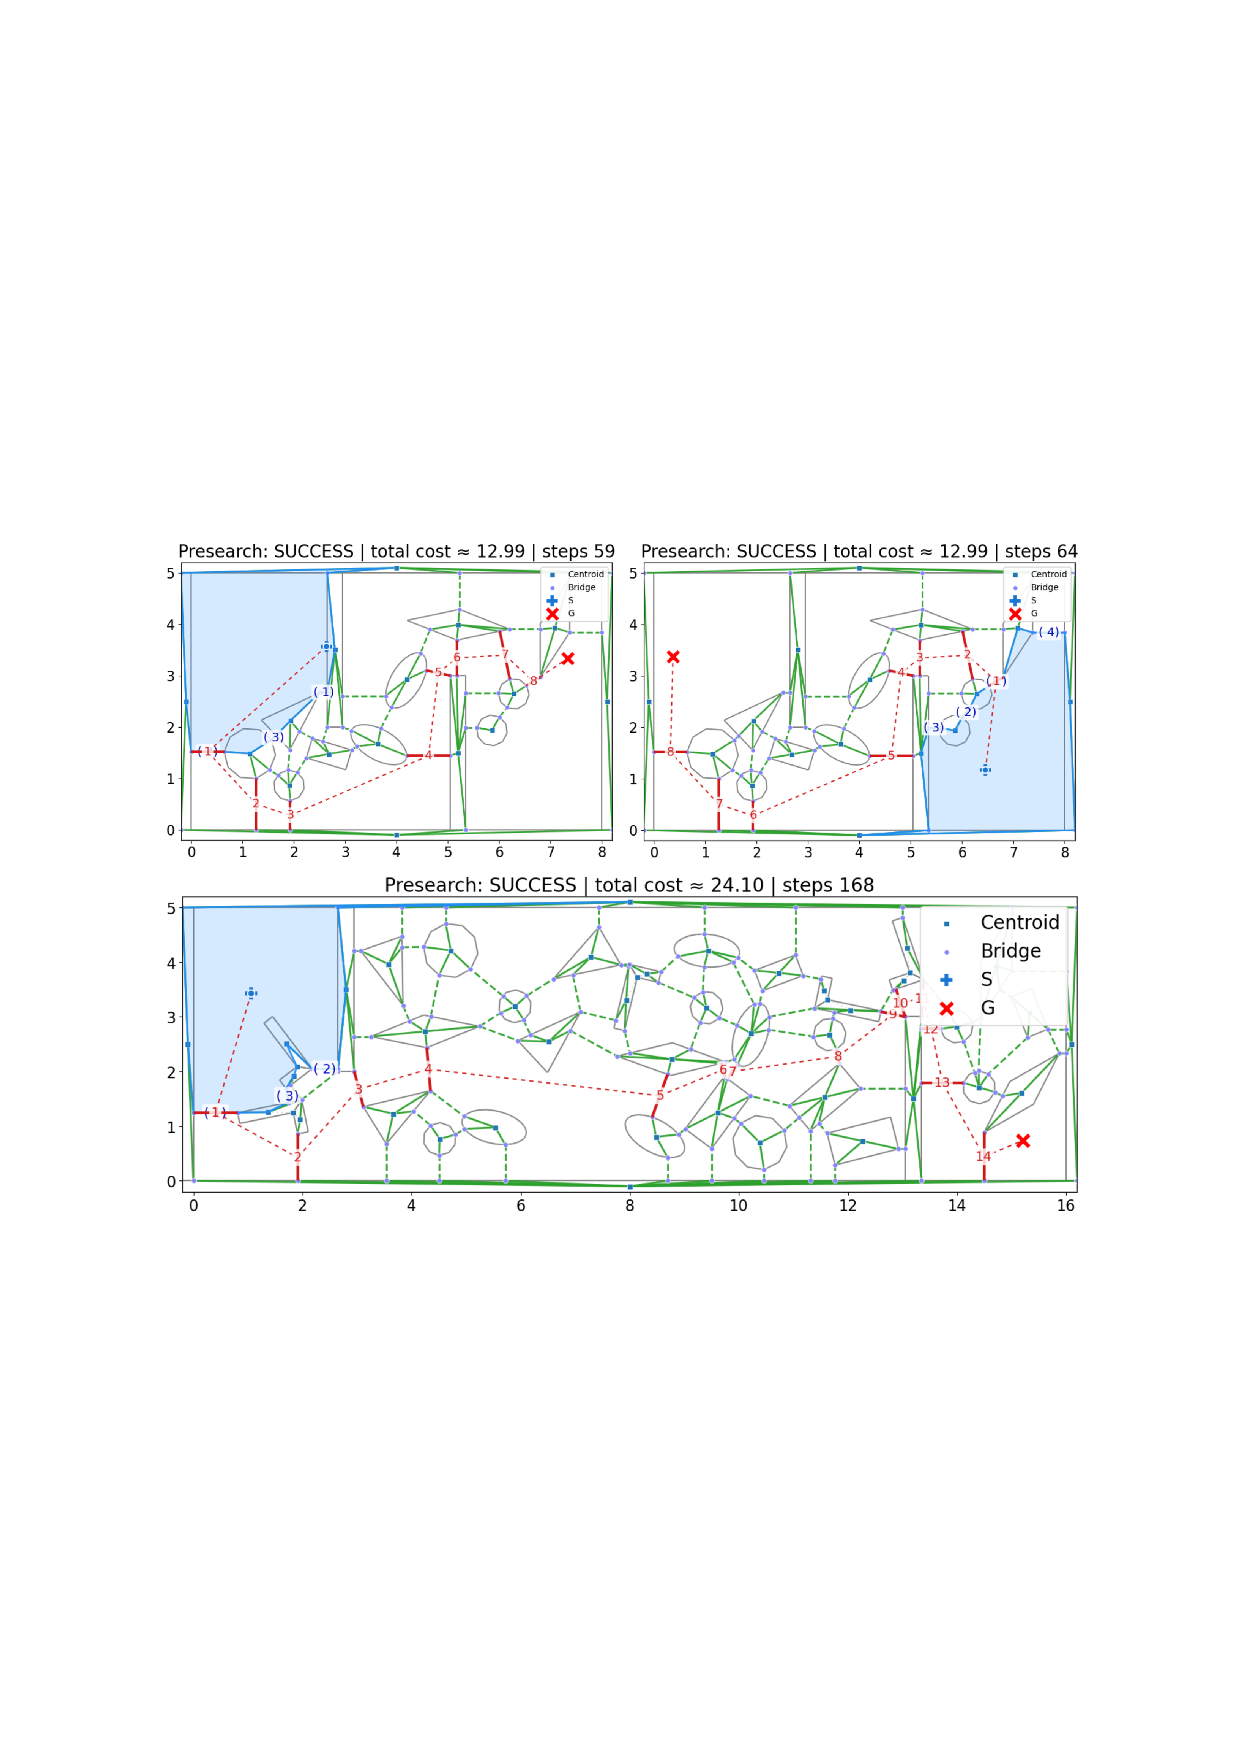
\includegraphics[width=\linewidth]{figures/presearch.pdf}% or {presearch.pdf}
  \vspace{-0.15in}
  \caption{
  Illustration for {the ranking of potential gaps.}
  Each panel overlays the WCCG together with the currently selected face (light blue).
  The algorithm (i) extracts the frontier loop from BugPlanner,
  (ii) enumerates candidate bridge--bridge gaps on the loop,
  (iii) assigns local first-hop ranks (blue numbers),
  and (iv) simulates a short presearch to predict the full gap-crossing sequence (red numbers).
  \textbf{Top:} identical environment with start and goal swapped;
  the resulting gap sequences are symmetric with identical predicted cost at $12.99$;
  \textbf{Bottom:} a larger map with about $30$ obstacles, where presearch returns a 14-gap sequence
  of predicted cost at $24.10$.
}

  \label{fig:presearch}
  \vspace{-0.1in}
\end{figure}
%------------------------------

\subsubsection{Long-term Cost w.r.t. Goal}
Furthermore, to prioritize gaps closer to the goal, a heuristic is added to the evaluation,
i.e.,
$h(g)=\eta\,\big\|\mathbf{o}(g)-\mathbf{s}_\texttt{V}^{\texttt{G}}\big\|$,
where $\eta>0$ is a scaling constant. Lastly, a short A$^\star$-style presearch virtually crosses
each candidate gap, recomputes the next frontier, and continues for a limited
beam width and depth. The predicted cost-to-connect is given by:
\begin{equation}\label{eq:pred_cost}
\widehat{\mathsf{Cost}}(g)\triangleq
\mathsf{C}\!\big(g \mid \mathcal{L},\mathbf{s}_{\mathcal{R}}\big)
+\!\!\!\sum_{g'\in\Pi^\star(g)}\!\!\!\big{\{}\mathsf{C}(g' \mid \cdot)+h(g')\big{\}},
\end{equation}
where $\Pi^\star(g)$ is the sequence of subsequent gaps discovered after
virtually crossing $g$;
the dots indicate updated inputs along that rollout;
and the scalar score $\widehat{\mathsf{Cost}}(g)>0$ for each candidate gap.
Consequently,
the final output of this module is the ranked list of candidate gaps, i.e.,
$\textsf{Rank}\big(\Gamma_\mathcal{L}\big)
\triangleq \textbf{argsort}_{g\in\Gamma_\mathcal{L}}\widehat{\mathsf{Cost}}(g)$,
which sorts $\Gamma_\mathcal{L}$ in ascending predicted cost. This
ordered set is passed to the hybrid search module, such that only the
promising gaps are expanded first.

\begin{remark}[Practical Improvement]\label{remark:gap}
Efficiency of the above ranking procedure can be improved by
caching frontier loops, storing the transitions
$(\mathcal{L},g)\mapsto\mathcal{L}'$, and accelerating the edge queries with
axis-aligned bounding-box culling. With a small beam width and depth
(typically around $8$), the runtime of ranking remains negligible compared to
the cost of simulation-based validation. \hfill$\blacksquare$
\end{remark}




%% %------------------------------
%% \begin{algorithm}[t]
%% \small
%% \caption{Frontier Presearch for Gap Ranking (compact)}
%% \label{alg:gap-ranking}
%% \DontPrintSemicolon
%% \SetKwInOut{Input}{In}\SetKwInOut{Output}{Out}
%% \Input{$\mathbf{s}^{\texttt{S}}$, $\mathbf{s}^{\texttt{G}}$, WCCG, $\lambda_{\mathrm{trans}}$, $\lambda_{\mathrm{push}}$}
%% \Output{First-hop gaps ranked by predicted cost}
%% $(\mathcal{L},\texttt{conn})\!\leftarrow\!\texttt{BugFrontier}(\mathbf{s}^{\texttt{S}},\mathbf{s}^{\texttt{G}})$;\;
%% \If{\texttt{conn}}{\Return $\emptyset$}
%% $\mathcal{C}\!\leftarrow$ bridge–bridge gaps on $\mathcal{L}$;\;
%% \For{$g\in\mathcal{C}$}{
%%   $J_1\!\leftarrow\!\lambda_{\mathrm{trans}}\mathsf{C}_{\mathrm{trans}}+\lambda_{\mathrm{push}}\kappa(g)[\max(0,W-w(g))+\delta]$;\;
%%   $(\texttt{succ},J_{\mathrm{tail}})\!\leftarrow\!\texttt{PresearchAfter}(g)$;\;
%%   $\widehat{\mathrm{Cost}}(g)\!\leftarrow\!J_1+\big(\texttt{succ}?J_{\mathrm{tail}}:\infty\big)$;\;
%% }
%% \Return $\mathrm{argsort}_{g\in\mathcal{C}}\widehat{\mathrm{Cost}}(g)$ (asc.)\;
%% \end{algorithm}

% %% ========================================
\begin{algorithm}[t]
\small
\caption{SiLS with Deferred Expansion (clean version)}
\label{alg:SiLS}
\DontPrintSemicolon
\SetKwInOut{Input}{In}\SetKwInOut{Output}{Out}
\SetKwFunction{Build}{BuildWCCG}
\SetKwFunction{Frontier}{BugPlannerFrontier}
\SetKwFunction{Rank}{PresearchRank}
\SetKwFunction{Predict}{SimPredict}
\SetKwFunction{Next}{NextBatch}

\Input{$\mathbf{s}^{\texttt{S}}$, $\mathbf{s}^{\texttt{G}}$, $W$, initial snapshot, batch size $B$}
\Output{Executable push plan or \texttt{fail}}

\BlankLine
\textbf{State of a node:} $\nu=(\texttt{snap}, \texttt{plan}, g, \mathcal{C}, j)$,
with candidates $\mathcal{C}$ (ranked) and cursor $j$.\;

\BlankLine
\textbf{Init:} $\nu_0\!\leftarrow\!(\texttt{snap}_0,\emptyset,0,\varnothing,0)$;\;
$\texttt{PQ}\!\leftarrow\!\{(\nu_0, f=\widehat{\mathsf{Cost}}_{\text{to-go}}(\texttt{snap}_0))\}$\;

\While{\texttt{PQ} not empty}{
  Pop $(\nu,f)$ with minimal $f$; \tcp*{$\nu=(\texttt{snap},\texttt{plan},g,\mathcal{C},j)$}
  \If{$\mathcal{C}=\varnothing$}{
    $(\texttt{connected}) \leftarrow \Build(\texttt{snap})$;\;
    \If{\texttt{connected}}{\Return \texttt{plan}}
    $\mathcal{L}\leftarrow \Frontier(\mathbf{s}^{\texttt{S}},\mathbf{s}^{\texttt{G}})$;\;
    $\mathcal{C}\leftarrow \Rank(\mathcal{L})$;\; $j\leftarrow 0$\;
  }
  $\mathcal{B}\leftarrow \Next(\mathcal{C}, j, B)$;\; $j\leftarrow j+|\mathcal{B}|$\;

  \ForEach{$\tau\in\mathcal{B}$ \textbf{in parallel}}{
    $(\texttt{ok}, \texttt{snap}', t_\text{push}) \leftarrow \Predict(\tau)$\;
    \If{\texttt{ok}}{
      $g' \leftarrow g + \mathsf{C}_{\mathrm{trans}} + t_\text{push}$;\;
      $h' \leftarrow \widehat{\mathsf{Cost}}_{\text{to-go}}(\texttt{snap}')$;\;
      Push $\big((\texttt{snap}',\,\texttt{plan}\!\cup\!\{\tau\},\,g',\,\varnothing,\,0),\, f'=g'+h'\big)$ into \texttt{PQ}\;
    }
  }
  \If{$j<|\mathcal{C}|$}{reinsert current $\nu$ into \texttt{PQ} with the same $f$}
}
\Return \texttt{fail}\;
\end{algorithm}


%==============================================
\subsection{Physics-Informed Hybrid Search}\label{subsec:simloop}

The hybrid search couples high-level decisions about blocking gaps with
low-level feasibility of multi-robot pushing. Unlike purely geometric
planners, this procedure simultaneously determines a sequence of gaps to clear
and physically feasible pushing actions, including directions, contact modes,
and forces. Parallel physics simulation is embedded so that many candidate
push strategies can be evaluated simultaneously at each expansion, and the resulting
successor states are returned to the search. This tight coupling of discrete
graph reasoning with continuous pushing dynamics is unique for the considered problem.

\subsubsection{Tree and Initialization}
The search tree $\mathcal{T}$ is composed of nodes
$\nu\triangleq(\mathbf{s},\pi)$, where $\mathbf{s}$ is the current system
state including the positions and orientations of all robots and movable
obstacles as in~\eqref{eq:transition}, and $\pi$ is the partial pushing
strategy realized so far as in~\eqref{eq:schedule}. Two global functions are
maintained: $\mathsf{Rank}(\nu)$ stores a ranked list of candidate gaps at this
node together with their exploration status, derived from~\eqref{eq:pred_cost};
and $\chi(\nu)$ returns the cumulative execution cost
from the root to $\nu$.
The root is initialized as
$\nu_0\triangleq(\mathbf{s}_0,\emptyset)$, where
$\mathbf{S}^{\texttt{S}}$ corresponds to the initial system state
$\mathbf{s}_0$. At initialization, $\chi(\nu_0)=0$, and
$\mathsf{Rank}(\nu_0)$ is constructed by first computing the frontier loop
$\mathcal{L}_\nu$ associated with~$\mathbf{s}_0$, then extracting the visible
gaps $\Gamma_{\mathcal{L}_\nu}$, and finally ranking them by their predicted
cost-to-connect.

\subsubsection{Node Selection}
At each iteration, the node with minimum best-first priority is selected from
the queue. The priority function balances the realized execution cost and the
estimated effort of remaining gaps:
\begin{equation}\label{eq:priority}
  f(\nu)\triangleq \chi(\nu)+\underset{g\in \textsf{Rank}(\nu)}{\textbf{min}}
  \widehat{\mathsf{Cost}}(g),
\end{equation}
where $\chi(\nu)$ is the cumulative execution cost so far, and the second term
is the minimum predicted remaining cost among the unexplored gaps of~$\nu$.
This scoring ensures that nodes are expanded in an order that jointly accounts
for physical effort already incurred and the most promising future actions.

\subsubsection{Node Expansion with Parallel Simulation}
When a node $\nu$ is selected for expansion, a batch of \emph{pushing
strategies} from $\mathsf{Rank}(\nu)$ is evaluated in parallel by simulation.
Each pushing strategy is defined as
\(\tau\triangleq(g,\mathbf{v},\boldsymbol{\xi})\), where
$g\in \boldsymbol{\Omega}$ is the chosen gap;
$\mathbf{v}\triangleq(v_x,v_y,\omega)\in \mathbb{R}^3$ is a short-horizon body
velocity for the manipulated obstacle;
and $\boldsymbol{\xi}\triangleq (\mathcal{C}_m,\mathbf{u}_m) \in (\partial\Omega_m)^N \times \mathbb{R}^{2N}$
is a contact mode specifying robot contact points and pushing forces as in~\eqref{eq:transition}.
Moreover, each candidate $\tau$ is first checked by a geometric quick-pass. If it passes,
it is evaluated by the simulator with the current state and pushing strategy:
\begin{equation}\label{eq:sim}
  (\mathbf{s}',\, \delta_\texttt{T},\, \delta_{\texttt{J}}) \triangleq \mathsf{EvalSim}
  \big{(}\nu,\, (g,\mathbf{v},\boldsymbol{\xi})\big{)},
\end{equation}
where $\mathbf{s}'$ is the successor state; $\delta_\texttt{T}>0$ is the time
cost; and $\delta_\texttt{J}$ is the control effort as in~\eqref{eq:problem}.
Thus, a successful evaluation produces a child
$\nu'\triangleq (\mathbf{s}',\pi')$, where $\pi'$ is obtained by appending
$\pi$ with $\tau$. The incremental realized cost of $\tau$ is
$\widehat{\mathsf{C}}(\nu,\,\tau)\triangleq \delta_\texttt{T} + \alpha\, \delta_\texttt{J}$,
with $\alpha>0$ the same trade-off parameter as in~\eqref{eq:problem}. The
cumulative cost is then updated by
$\chi(\nu')\triangleq \chi(\nu)+\widehat{\mathsf{C}}(\nu,\,\tau)$. Since many
pushing strategies are simulated concurrently, numerous successors can be
expanded in parallel at each iteration.

\subsubsection{Termination}
Termination occurs when a node $\nu$ reaches a state $\mathbf{s}$ for which a
$W$--clear path $\mathcal{P}^W_\texttt{V}$ exists from
$\mathbf{s}_\texttt{V}^{\texttt{S}}$ to $\mathbf{s}_\texttt{V}^{\texttt{G}}$,
as certified by~\eqref{eq:wccg_criterion}. In this case, the schedule $\pi$
stored in $\nu$ constitutes a complete solution to~\eqref{eq:problem}, encoding
both the sequence of gaps to clear and the physically feasible pushing actions
that realize them.

\begin{remark}[Parallel Expansion and Mode Reuse]\label{remark:simloop}
Efficiency of the hybrid search stems primarily from parallel evaluation of
pushing strategies, which allows many candidate futures to be simulated at once
for each expansion. Deferred expansion ensures that nodes with long candidate
lists remain in the priority queue until all tasks are attempted, preventing
search starvation. In addition, validated $(\boldsymbol{\xi},\mathbf{v})$ pairs
are cached locally within a subtree and stored in a persistent ModeTable for
reuse across similar obstacles, significantly reducing repeated physics calls.
These mechanisms yield orders-of-magnitude speedup relative to naive
simulation-based search. \hfill$\blacksquare$
\end{remark}

% %%========================================
%==============================
\subsection{Overall Analyses}\label{subsec:overall}


%==============================================
\subsubsection{Online Execution and Adaptation}\label{subsec:execute}

Once the hybrid pushing plan $\nu^\star$ is generated, the robot fleet executes the task
in real-time by following the guiding path $\overline{\mathbf{S}} = \{\mathbf{s}_0, \dots,
\mathbf{s}_L\}$. Each robot tracks the assigned trajectory segments, pushing the target
along the planned path while adjusting its motion based on the current target state
$\mathbf{s}_m(t)$ and interaction mode $\xi_n(t)$. The robots apply the desired forces
at the contact points $\mathbf{c}_n(t)$ using the control law:
\[
  \widehat{\mathbf{v}}_n = K_{\texttt{vel}} \left(\widehat{\mathbf{c}}_n - \mathbf{c}_n\right), \quad
  \widehat{\omega}_n = K_{\texttt{rot}} \left(\widehat{\psi}_n - \psi_n\right),
\]
to guide the object from the start to the goal while ensuring contact force consistency.
Transitioning between obstacles is handled according to the hybrid plan. Specifically,
as each robot pushes the object, it follows a **collision-free path** to the next set of
contact points on the next obstacle, ensuring that all movement respects the planned
interaction modes, and the sequence of obstacles is maintained. This transition is dynamically
adjusted as the robots continue pushing the target toward the goal.

In case of failures, such as when the object deviates from its expected position,
the algorithm triggers adaptation. If the object fails to reach the desired position,
the system checks the tracking error:
\[
  \mathrm{dist}(\mathbf{s}_m(t'), \varrho_\ell) \geq \delta_{\texttt{f}}, \quad
  \|\mathbf{s}_m(t') - \mathbf{s}_m(t'')\| < r_{\texttt{stuck}},
\]
and re-computes the entire hybrid plan based on the current system state. This includes
recalculating the sequence of movable obstacles to push, the contact points, and the
pushing forces to be applied. The updated plan is then executed with the control law in
\eqref{eq:control} to guide the robots toward the goal despite disruptions, ensuring
the task is completed even under unforeseen circumstances.



%==============================
\subsubsection{Complexity Analysis}\label{subsubsec:complexity}

The time complexity of the proposed method is dominated by three main components: the W-Clearance
Connectivity Graph (WCCG), gap-ranking strategy, and simulation-in-the-loop hybrid search. Constructing
the WCCG has a complexity of $\mathcal{O}(M^2 \log M)$, where $M$ is the number of movable obstacles,
due to the graph search and clearance checks. The gap-ranking strategy, which involves evaluating each
critical gap and ranking them based on their clearance and the obstacles’ mass, has a complexity of
$\mathcal{O}(G \log G + G M)$, where $G$ is the number of critical gaps and $M$ is the number of obstacles.
The most computationally intensive part is the simulation-in-the-loop hybrid search, which checks the feasibility
of each mode by simulating robot dynamics. The complexity for each simulation step is $\mathcal{O}(N^{3.5})$, where
$N$ is the number of robots, and the overall complexity of the hybrid search is $\mathcal{O}(N^{3.5} \cdot M \cdot L)$,
where $L$ is the number of keyframes in the path. Hence, the overall complexity is primarily determined by the hybrid
search algorithm.




%==============================
\subsubsection{Generalization}\label{subsec:general}

The proposed framework can be generalized in several directions. (I) \emph{Heterogeneous robots}:
When robots have varying capabilities, such as different maximum forces, the hybrid plan $\nu^\star$
should be adjusted by assigning more powerful robots to obstacles that require higher forces,
with smaller robots handling less demanding tasks. This adjustment is reflected in the interaction modes
$\boldsymbol{\xi} = (\mathbf{c}_1, \mathbf{f}_1, R_1), \dots, (\mathbf{c}_N, \mathbf{f}_N, R_N)$,
where $\mathbf{f}_n$ represents the force for each robot. (II) \emph{Simultaneous clearing}:
The framework can be extended to allow multiple obstacles to be pushed simultaneously,
improving the efficiency of path clearing. This requires modifying the WCCG, $\mathcal{G}^W(t)$,
to support parallel tasks and ensuring collision-free paths for multiple robots. (III) \emph{Dynamic
obstacle movement}: The method can handle dynamic obstacles by incorporating real-time sensor data
and updating the WCCG, allowing the hybrid search algorithm in Section~\ref{subsec:simloop} to adapt the plan
on-the-fly to avoid collisions and clear the path efficiently, even with moving obstacles.

% %%========================================
